\documentclass[oneside]{VUMIFPSkursinis}
\usepackage{algorithmicx}
\usepackage{algorithm}
\usepackage{algpseudocode}
\usepackage{amsfonts}
\usepackage{float}
\usepackage{amsmath}
\usepackage{bm}
\usepackage{caption}
\usepackage{color}
\usepackage{float}
\usepackage{graphicx}
\usepackage{listings}
\usepackage{subfig}
\usepackage{wrapfig}
\usepackage[%  
    colorlinks=true,
    linkcolor=black
]{hyperref}
\university{Vilniaus universitetas}
\faculty{Matematikos ir informatikos fakultetas}
\department{Programų sistemų katedra}
\papertype{Laboratorinis darbas I}
\title{Automatinė ūkio valdymo sistema}
\titleineng{Automatic farm management system}
\status{2 kurso 3 grupės studentai}
\author{Matas Savickis}
\secondauthor{Justas Tvarijonas}  
\thirdauthor{Greta Pyrantaitė}   
\fourthauthor{Rytautas Kvasinskas}
\supervisor{Karolis Petrauskas, Doc., Dr.}
\date{Vilnius – \the\year}

% Nustatymai
%\setmainfont{Palemonas}   % Pakeisti teksto šriftą į Palemonas (turi būti įdiegtas sistemoje)
\bibliography{bibliografija}

\begin{document}
\maketitle

\tableofcontents


\centering	
\sectionnonum{Įvadas}
Automatinė ūkio valdymo sistema(toliau Auto ūkis) - yra programa leidžianti ūkininkui valdyti jo ūki skaitmeniniu būdu. Auto ūkis  leidžia stebėti kiekvieno individualaus gyvūno bioparametrus(kraujo spaudima, svorį, sveikatą), ūkio technikos judėjimą po žemės plota, gyvūnų registracija. Taip pat sistema vartotojui leidžia sekti dirvos parameturs(drėgmę, pH lygi),  oro prognozes ir aplinkinių teritorijų gyvūnų ligų paplitimą. Auto ūkis padeda ir su verslo valdymu, nesunkiai galima samdyti darbuotojus, atlikti buhalterinę apyskaita, stebėti rinkos kainas ir skaičiuoti bei numatyti galimą pelną. Iškilus nelaimės per Auto ūkio sistemą galima greitai iškviesti greitąją pagalba, policiją, gaisrinę ar saugos tarnybą. Orai prognozės yra paimtos iš www.gismeteo.lt. Pagrindinė sistemos inovacija yra tai, kad kai sistema yra pilnai įdiegta darbuotojų skaičius palaikyti ūki tampa minimalus. Ūkio technika būtų valdoma automatiškai todėl vairuotojų ir derliaus nurikėjų nereiktų. Gyvūnų sekimas yra įgyvendinamas microkontrolerio Arduino pagalba. Kadangi šis kontroleris ledidelis ir lengvai pritaikomas visiokio pobūdžio darbams ji kartu su WiFi moduliu sistema naudoja gauti gyvųno lokacija per Google maps. Taip pasiklydę ar pavogti gyvųnai būtų greitai gražinami surandami ir gražinami. Žemės laistymas, tręšimas taip pat būtų automatizuotas, parametrai gaunami per Arduino detektorius, kurie pagal pasikeitusia dirvos kompozicija nusprendžia ko trūksta žemei ir aktyvuoja laistymo ir tręšimo sistemas. Darbuottojų samdymas yra įgyvendintas per darbo biržos puslapį, kur greitai ir nesunkiai galimą įdėti skelbimą arba surasti darbuotoją. Buhalterija yra tvarkoma nemokamos buhalterijos programos Wave Accounting kuri yra implementuota į Auto ūki.  Auto ūkio sistema yra parašyta JAVA kalba kas leidžia programą paleisti ant betkurios operacinės sistemos. Ateityje numatoma galimybė programą perkelti į išmaniuosius telefonus. Sistema buvo projektuojama pasitelkiant www.planttext.com ir www.draw.io funkcionalumą.

\sectionnonum{Žodynas}
\begin{itemize}
	\item Klasės:
		\begin{itemize}
			\item[*] AutoŪkis - pagrindinė(main) programos klasė. Ši klasė piešia grafinę vartotojo sąsaja ir laiko savyje kitų klasių objektus kurių informacija reikalinga piešimui
			\item[*] Map - teritorijos piešimui skirta klasė.
			\item[*] ŽemėsTeritorija - apskaičiuoja tam tikros teritorijos plotą.
 			\item[*] Gyvūnas - klasė skirta gyvūno rodmenims ir metodams saugoti
			\item[*] AriamasLaukas - laiko savyje reikšmes apibūdinančias unikalų lauką ir metodus susijusius su lauko darbu.
			\item[*] Ganykla - laiko parametrus ir metodus darbui su ganyklomis kurios yra žemės plote.
			\item[*] ŪkinisPastatas - saugo ūkinius 
			\item[*] ŪkioTechnika - laiko ūkio technikos charakteristikos reikšmes. Apskaičiuoja technikos judėjimo greitį.
			\item[*]Žemės parametrai - saugo įvairius žemės parametrus(drėgmė, ph...).
			\item[*] Orai - klasė skirta pasiimti orų prognozes iš www.gismeteo.lt kurių paprašo vartotojas.
			\item[*] Žemės detektorius - klasė skirta bendrauti su žemės detektoriumi

		\end{itemize}
	\item Bendri terminai:
		\begin{itemize}
			\item[*] Žemės plotas - vieta kurią valdo ir gali stebėti vartotojas(ūkininkas) 
			\item[*] Detektorius - Arduino mikro kontroleris
			\item[*] Ūkininkas - žmogus kurio valdomoje teritorijoje įdiegtas Auto ūkis
			\item[*] Arduino - mikrokontroleris skirtas ūkio sekimui
			\item[*] Automašiskai valdoma - nereikalinga žmogaus pagalba
			\item[*] Darbuotojas - žmogus dirbantis ūkininko versle
			\item[*] Gyvūnas - visi gyvūnai kurie priklauso ūkininkui ir yra registruoti Auto ūkis sistemoje 
		\end{itemize}
\end{itemize}

\section{Sukurtos sistemos aprašymas(v1.0)}

\subsection{Loginis pjūvis}
Pagal suprogramuotą šabloninį programos karkasą nubraižėme  \hyperref[fig:uml]{\textit{ UML diagramą}} minėta PlnatText programa.

	\begin{figure}[H]	
	\centering	
		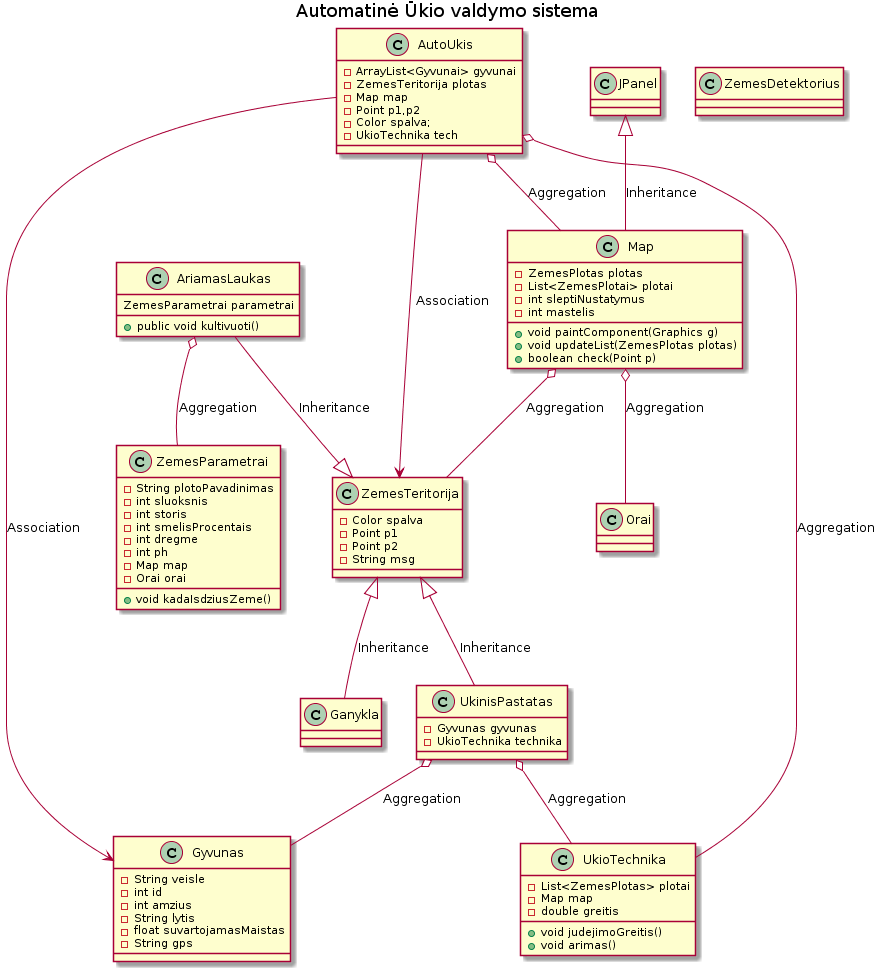
\includegraphics[width=\textwidth,height=\textheight,keepaspectratio]{uml.png}	
		\caption{}
		\label{fig:uml}
	\end{figure}

	\pagebreak
	\begin{itemize}
		\item Dizainas: 
		\begin{itemize}
			\item Pagrindinė klasė yra AutoUkis.form. Joje sukurtas ir aprašytas Graphical User Interface (GUI), visas vartotojo bendravimas su programa vyksta per ją, nes per ją pasiekiami visi duomenys iš kitų klasių, pavyzdžiui duomenys, esantys klasėje Gyvūnas, kurioje įrašoma vartotojo įvesta informacija apie gyvūną (veislė, amžius, t.t.). Taip pat AutoUkis klasėje kuriama dauguma objektų ir jie ten laikomi, sudedami į sąrašus. Visos kitos klasės turi savo atskiras paskirtis, tokias kaip žemėlapio braižymas, oro prognozių sekimas ir įvairių parametrų laikymas. Kai kurios klasės (pvz. ZemesDetektorius) buvo sukurtos vėlesniam panaudojimui, bet šiuo metu nėra niekur panaudotos.
Dėl to, ką būtų buvę galima daryti kitaip, GUI perkėlimas į atskirą klasę padarytų programą skaitomesnę ir tvarkingesnę, būtų lengviau rasti atskirą kodą. Dar viena alternatyva būtų įgyvendinti front-end dalį web aplinkoje, bet šiuo metu nematome tam būtinybės.
		\end{itemize}
		\item Funkcionalumas:
		\begin{itemize}
		\item Viso užsibrėžto programos funkcionalumo įgyvendinti nepavyko. Kai kurios klasės buvo sukurtos ateityje planuojamoms funkcijoms, kurios dar nėra implementuotos. Programa kol kas veikia tik ant kompiuterio ir vienintelis jos bendravimas su internetu yra per Orai klasę, kuri skirta vartotojo pasirinkto miesto orų prognozėms gauti iš gismeteo.lt svetainės. Klasėse Gyvunas, Map, ZemesTeritorija ir iš jos išeinančiose klasėse saugomi atitinkami duomenys apie sukurtus objektus bei aprašyti dar neišplėtoti metodai, tokie kaip žemės teritorijos žymėjimas. Planuojama, kad klasė ZemesDetektorius generuos atsitiktinius parametrus, kurie bus perduoti ZemesParametrai klasei.
Nepilnai įgyvendintas finkcionalumas ir neišbaigtos klasės sukelia nepatogumų aprašant programą, nes sunku braižyti diagramas, suvokti aiškius ryšius tarp komponentų ir vykdomas funkcijas.
		\end{itemize}	
	\end{itemize}
	\pagebreak
\subsection{Kūrimo pjūvis}
\begin{itemize}
\item Dizainas: 
		\begin{itemize}
			\item Pradėjus rašyti programą nepagalvojome apie kūrimo pjūvį ir kaip teisingiau būtų pradėti viską. Žiūrint dabar visa programa buvo pradėta kurti pagal Bottom -> Up principą. Iš pradžių apsirašėme daugybę mažų klasių ir paskui jas bandėme apjungti į didesnę sistemą. Išskyrėme tokius komponentus kaip ūkininkas, programa, orų tarnyba, žemės detektorius ir administratorius. Kiekvienas komponentas turi skirtingas prieigas prie informacijos ir skirtingas funkcijas, reikalingas ūkio visapusiškam funkcionavimui. Kai kurios klasės liko nepanaudotos, nes šiuo metu jos neatrodo pakankamai svarbios pradiniam projekto variantui. Ūkiniko, Admin ir darbuotojo panelės įtrauktos į dokumentaciją norint pavaizduoti skirtingas prieigas prie sistemos.
		\end{itemize}
		\end{itemize}
\begin{figure}[H]
\centering	
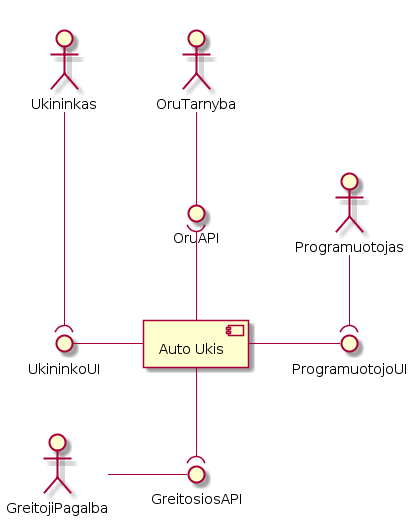
\includegraphics[width=10cm,height=15cm,keepaspectratio]{l0.png}	
\caption{}
\label{fig:l0}
\end{figure}
	\begin{itemize}
		
		\item \hyperref[fig:l0]{\textit{L0}}:
		\begin{itemize}
			\item  \hyperref[fig:l0]{\textit{Šioje diagramoje}} pavaizdavome sistemos bendravimą su išoriniais agentais tokiais kaip Greitoji pagalba, Ūkininkas ir t.t. . Ši diagrama aiškiai ir paprastai parodo kuriamus ir įgyvendinamus interfeisus. Galbūt būtų galima Greitosios Pagalbos interfeisą išskaidyti į kelis detalesnius interfeisus, bet apskritai didelių problemų nepastebime.

		\end{itemize}

	\end{itemize}
\begin{figure}[H]	
\centering	
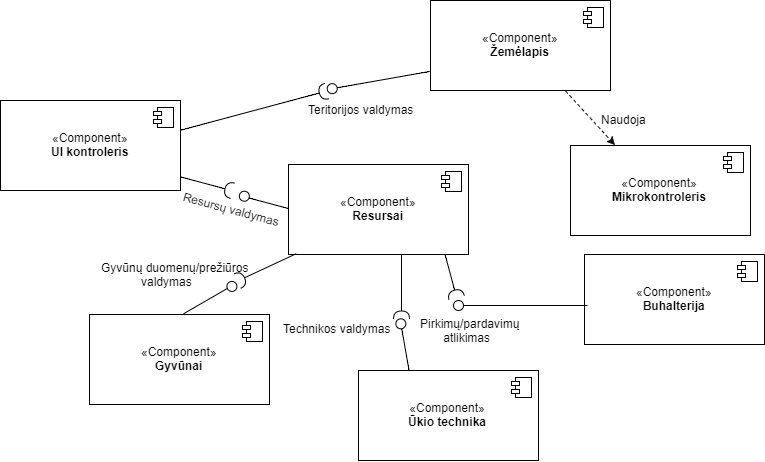
\includegraphics[width=14cm,height=14cm,keepaspectratio]{l1.png}	
\caption{}
\label{fig:l1}
\end{figure}

\begin{itemize}
	\item L1: Sudėjus komandos idėjas apie tai, kaip turėtų atrodyti \hyperref[fig:l1]{\textit{ L1 diagrama}}, supratome, kad mūsų sistema neturi normalios struktūros ir gerai nebuvome pagalvoję kaip visi komponentai siesis vieni su kitais, todėl ir diagrama atrodo chaotiška. Trūksta konkretumo kaip turi Admin sietis su kitas komponentais. Programa atsiranda kaip komponentas  kas greičiausiai yra nekorektiška.

\end{itemize}
\begin{figure}[H]
\centering	
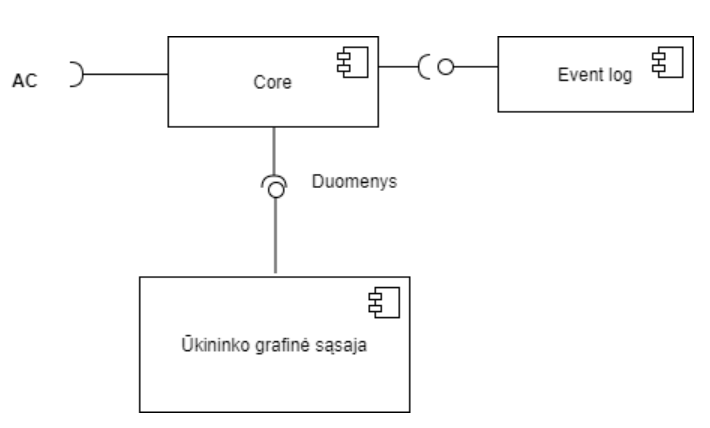
\includegraphics[width=10cm,height=10cm,keepaspectratio]{l2uki.png}
\caption{}
\label{fig:l2uki}
\end{figure}
	

	\begin{itemize}
		\item L2(Ūkininkas):\hyperref[fig:l2uki]{\textit{  Šioje diagramoje}} parodyta, kad programos pagrindas kuria suteikia interface’a grafinei vartotojo sąsajai. Paduoti duomenys yra užregistruojami Event Log’e.

	\end{itemize}
	\begin{figure}[H]
	\centering	
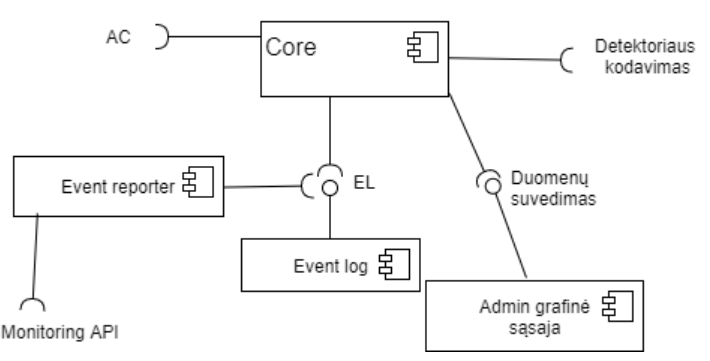
\includegraphics[width=10cm,height=10cm,keepaspectratio]{l2admin.png}
\caption{}
\label{fig:l2admin}
\end{figure}
	
	
	\begin{itemize}
		\item L2(Admin)\hyperref[fig:l2admin]{\textit{  Šioje diagramoje}}  parodyta,kad programos pagrindas naudoja duomenų suvedimo interface, kurį suteikia admin grafinė sąsaja, bei naudoja Detektoriaus kodavimo interface. Visus įvykius įrašo į event log

	\end{itemize}
	\begin{figure}[H]
	\centering	
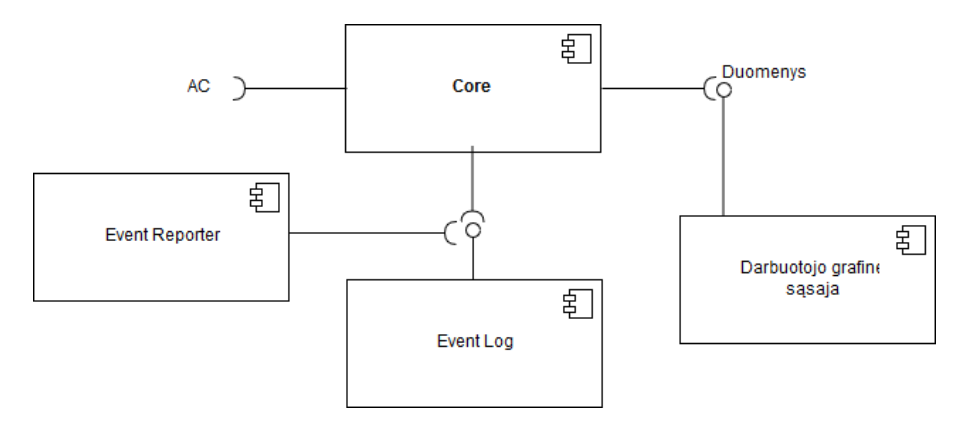
\includegraphics[width=10cm,height=10cm,keepaspectratio]{l2darb.png}
\caption{}
\label{fig:l2darb}
\end{figure}
		

\begin{itemize}
		\item L2(Darbuotojas):\hyperref[fig:l2darb]{\textit{  Šioje diagramoje}}  parodyta, kad programos pagrindas  grafinę sąsają ir perduoda duomenis į event log’ą. 
\end{itemize}
\begin{figure}[H]
\centering	
	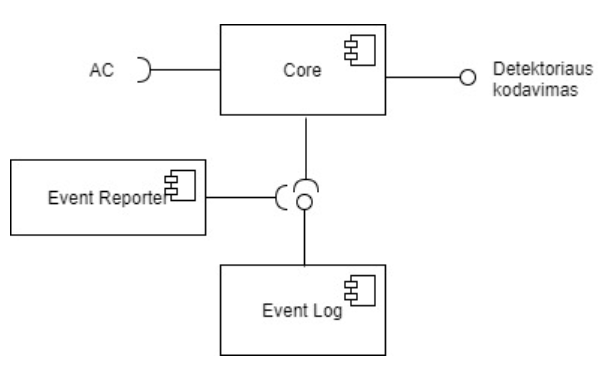
\includegraphics[width=10cm,height=10cm,keepaspectratio]{l2det.png}
	\caption{}
	\label{fig:l2det}
\end{figure}
		
\begin{itemize}
		\item L2(Detektorius):\hyperref[fig:l2det]{\textit{ Ši diagrama}} vaizduoja detektoriaus išvedamus duomenis. Įvykiai įrašomi Event Log’e.
\end{itemize}
\pagebreak
		


\subsection{Use case}
\subsection{Proceso pjūvis}
	Šiame skyriuje parodoma programos elgsena jos vykdimo metu.
\subsubsection{Veiklos diagramos}
	Vaizduojama\hyperref[fig:ActivityMapŽimėjimas]{\textit{ žemėlapio žymėjimo veiklos diagrama}}. Nurodomi pagrindiniai žingsniai braižant žemėlapį.
	\vskip 0.5cm
	\begin{figure}[H]
	\centering	
	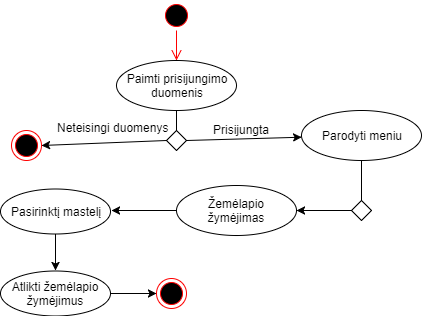
\includegraphics[width=10cm,height=10cm,keepaspectratio]{ActivityMapŽimėjimas.png}
	\caption{}
	\label{fig:ActivityMapŽimėjimas}
\end{figure}

	
\subsubsection{Būsėnų diagrama}
 \hyperref[fig:Busenu]{\textit{Šioje diagramoje}} parodomos galimos vartotojo būsenos ir keliai kaip tas būsenas pasiekti. Šiuo metu programoje tėra 2 būsenos, taigi diagrama yra labai paprasta.
	\begin{figure}[H]
	\centering	
	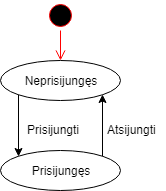
\includegraphics[width=5cm,height=6cm,keepaspectratio]{Busenu.png}
	\caption{}
	\label{fig:Busenu}
\end{figure}
\pagebreak
\subsection{Fizinis pjūvis}
	Šiame skyriuje parodoma šios sistemos techninė įranga, komunikacija, tačiau kadangi šioje šabloninėje versijoje nenaudojame kitų techninių resursų be kompiuterio, taigi fizinis pjūvis parodo tik nedidelį kiekį informacijos.
	\newline
	\vskip 0.5cm
	\begin{figure}[H]
	\centering	
	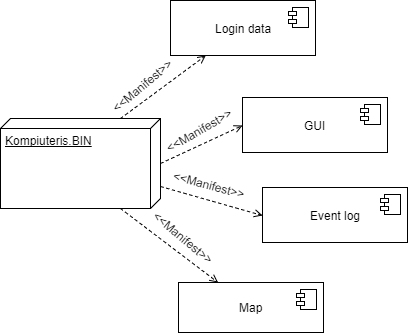
\includegraphics[width=10cm,height=10cm,keepaspectratio]{Deployment.png}
	\caption{}
	\label{fig:Deployment}
\end{figure}
	\begin{itemize}
		\item D0: \hyperref[fig:Deployment]{\textit{Šioje diagramoje}} parodyta, kas saugoma device kompiuteris. 
		Iš diagramos matome, kad šiame įrenginyje saugomi prisijungimo duomenys, Vartotojų grafinės sąsajos, teritorijos žemėlapis bei programoje atliktų veiksmų išrašas. Alternatyva buvo saugoti šiuos duomenis išnuomuotame web service, tačiau daug negalvoję nusprendėme duomenis saugoti kompiuteryje.

	\end{itemize}
		\begin{figure}[H]
		\centering	
	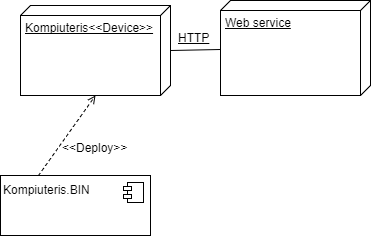
\includegraphics[width=10cm,height=10cm,keepaspectratio]{Deployment0.png}
	\caption{}
	\label{fig:Deployment0}
\end{figure}
	\begin{itemize}
		\item D1: Tai \hyperref[fig:Deployment0]{\textit{bendresnė D0 diagrama}}, joje matome, kad kompiuteris bendrauja su web HTTP ryšiu norėdamas gauti pranešimus apie orus.
	\end{itemize}

\section{Perprojektuotos sistemos aprašymas(To-Be, v2.0)}

\subsection{Loginis pjūvis}
\subsection{Kūrimo pjūvis}
\subsection{Use case}
\subsection{Proceso pjūvis}
\subsection{Fizinis pjūvis}



\sectionnonum{Rezultatai ir išvados}



\end{document}
